\chapter{Introduction}

\section{Motivation}

Unmanned Aerial Vehicles (UAVs) have proved their great capability in
transporting cable suspended loads in recent years. They offer the ability
to reach places that are dangerous or remote and can transfer equipment
that is otherwise difficult to move [1]. This can be of great utility
during rescue operations, construction, humanitarian aid and logistics.
While early efforts focused on single multirotors, they often face
engineering challenges due to their limited payload capacity, endurance and
ability to control the full load pose. To counter these challenges,
collaborative teams of multirotors have been proposed.

Multirotors were mainly used because they are more agile than fixed-wings
carriers and can hover. However, these solutions tackle only the limited
payload capacity and the full pose control problems. They still suffer
from reduced operational range due to their lower energy efficiency. On
the other hand, fixed-wings platforms offer better energy efficiency [2]
and thus longer operational range and higher cruising speeds. Hence,
fixed-wings platforms are better suited for applications that require long
range. This comes at the cost of a more complex control architecture
because fixed-wings carriers cannot simply hover in place.

Multiple fixed-wings UAVs need to coordinate among themselves in order to
allow the payload to stay stationary while they are loitering. This
coordination is also needed in many other scenarios in the trajectory
control of the payload. For this reason, most previous efforts were using
multirotors. Recent works by [3],[4] showed that it is possible to
calculate online coordinated trajectories. The solution however, was based
on a centralized controller that calculated all the trajectories and then
assigns each carrier its trajectory. Additionally, to calculate the
trajectories online it had to solve an NLP each time step. This makes
onboard deploying of the solution particularly challenging due to the high
computational cost.

In this work, we propose a decentralized solution based on Imitation
Learning (IL) and Multi-Agent Reinforcement learning (MARL). The proposed
solution also allows for onboard deployment as the computational cost per
step is greatly reduced to the inference time. Additionally, its
decentralized nature allows it to be deployed with great flexibility in
many applications.

\begin{figure}[htb]
  \centering
  % Both boxes are forced to the same width AND height (stretching each photo
  % to fit, aspect ratio not preserved) so the pair reads as one equal-sized
  % block rather than two mismatched rectangles.
  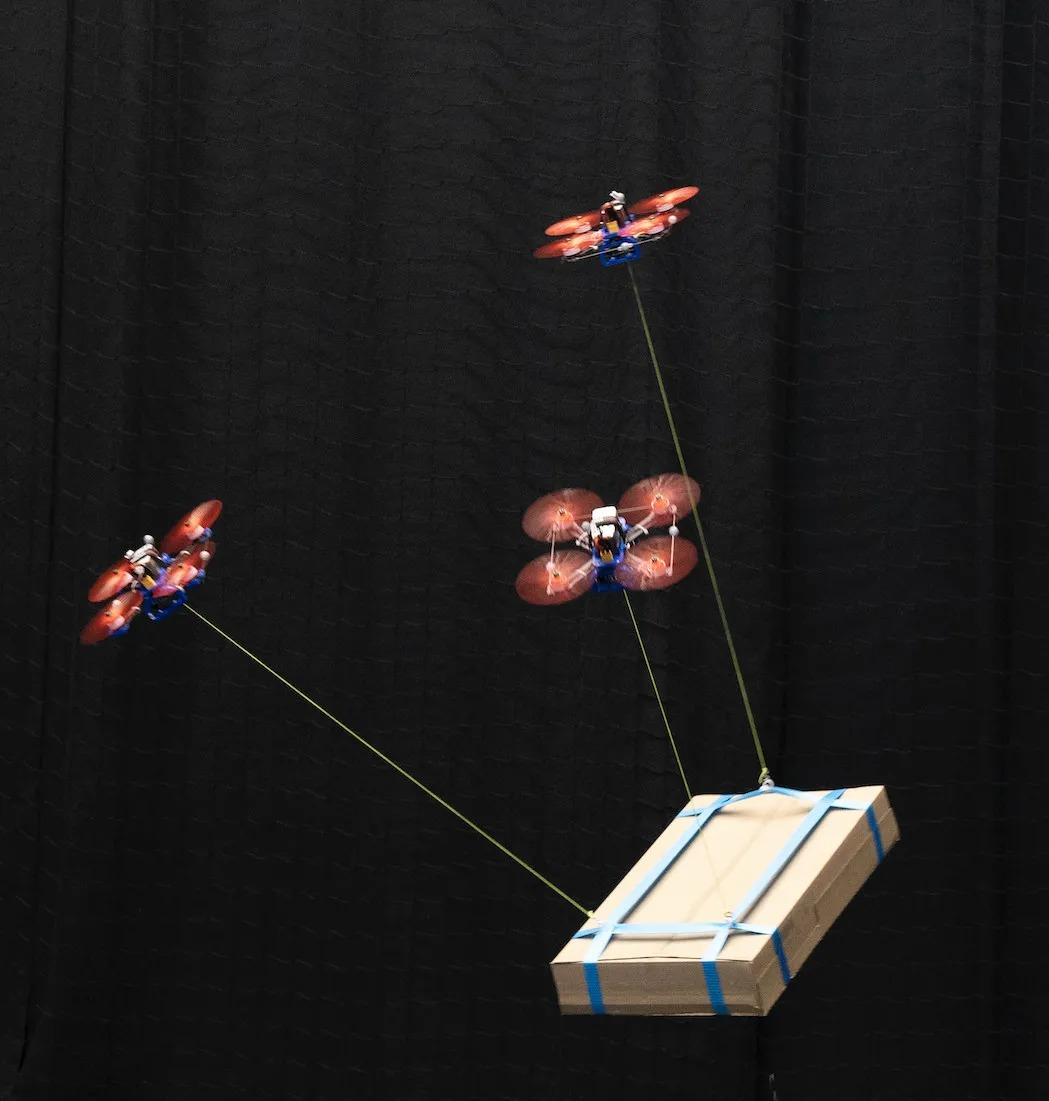
\includegraphics[width=7.7cm,height=10cm]{figures/fig-multirotors-1.jpg}%
  \hspace{0.6cm}%
  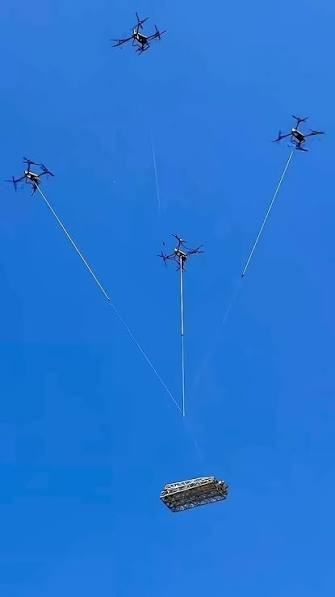
\includegraphics[width=7.7cm,height=10cm]{figures/fig-multirotors-2.jpg}
  \caption{Cooperative teams of multirotor UAVs transporting a cable-suspended payload.}
  \label{fig:multirotor-teams}
\end{figure}

\section{Main challenges}

Fixed-wings UAVs present a unique and underexplored challenge in that they
cannot hover. Since they always have to be moving, that means they will
apply additional forces and torques on the payload other than the desired
ones to move it along its trajectory. The main idea to solve this problem
is to have these additional forces (referred to as internal forces) 
cancel each other out such that only the desired wrench (forces and
torques) on the payload remains. 

Hence, coordination between the carriers is a requirement. However, this coordination 
can still be achieved
through well designed decentralized mechanisms depending on the load state
and other local observations, without the explicit need for 
inter-carrier communication or measurements.

Fixed-wings UAVs also present a subtle but nontrivial problem, since the
carrier needs to be always moving, the load state to carrier action map is not
a well-defined function. In other words, we can have the same load state
but different carrier actions in different times. Consequently, the carrier
needs to take decisions based on memory or some understanding of time.
Moreover, the actions of the carriers are not identical at the same moment in
time and at the same payload state. This is due to the fact that the
internal forces that will cancel each other need to be produced by
different carrier trajectories. 

Furthermore, since the policy is
decentralized, each carrier will have to make its own observation of the load.
We can imagine using an AprilTag on the load and each carrier has its own
camera that sees it. Hence, each observation is going to be subject to its own
noise and delay, leading to desynchronization in the load state between the
different carriers. Therefore, the policy needs to learn good actions with
limited and potentially outdated information. This naturally leads to a
Partially Observable Markov Decision Process (POMDP) problem formulation.
\_\_\_\_\_might add some sentences here about the history thing\_\_\_\_ .
Finally, the problem has many other aspects that are beyond the scope of
this thesis (e.g. enforcing a minimum turning radius).

The goal of this thesis is to answer whether a fully decentralized policy
(using a combination of learning-based and classical methods) is able to
coordinate the carrier trajectories even when they do not fully agree
on the state of the system. Instead of
relying on a centralized controller that has access to the full and true
state, can they still learn a reactive policy that is
able to stabilize the load and maintain their coordinated trajectories?
Taking into consideration the carriers have their own local heterogeneous 
asynchronous observations. Additionally, the policy must be lightweight enough to 
deploy onboard and execute in real time.
